\chapter{Pruebas y análisis de resultados}\label{cap:PruebasResultados}

Este capítulo ofrece los resultados del estudio experimental conducida en este trabajo. Es importante destacar que este capítulo está dividido en dos secciones, un \textbf{estudio de escalabilidad} donde se comprueba el comportamiento de los algoritmos en términos de convergencia cuando disponen de \textbf{100 mil} de evaluaciones de la función objetivo; a la vez, comprueba como evoluciona la convergencia en función del tiempo, de cara a establecer las evaluaciones de la función objetivo que serán conducidas en el \textbf{estudio experimental completo}, donde se obtendrán resultados más representativos al permitir que cada algoritmo ejecute \textbf{10 veces} cada problema.

Una sección dedicada al \textbf{análisis exhaustivo de los resultados} será conducida al final de la experimentación completa, donde se interpretan las soluciones de cada una de las técnicas y donde primará un enfoque de implementación real, lo que implica revisar la calidad de las soluciones obtenidas en términos de eficacia y eficiencia, teniendo en mente el objetivo que se busca desde el principio, que es trasladar el uso de las técnicas más potentes del campo LSGO a un entorno real.

\section{Estudio de escalabilidad}\label{sect:FE1}

Este estudio sirve para establecer de forma preliminar el comportamiento de los algoritmos frente a cada problema del EEG. Se resumen los primeros resultados en tablas temporales  donde se miden los \textbf{tiempos de ejecución} de cada algoritmo en relación al número de \textbf{evaluaciones de la función objetivo} que va ejecutando. De esta forma se identifican aquellos comportamientos que determinan la \textbf{posible validez} de un algoritmo de cara a formar parte de una solución real del problema del EEG. 

En esta fase, para cada algoritmo y subproblema del EEG, esto es, para cada dimensión tanto con ruido como sin éste, se exponen las tablas de resultados de tiempos junto con la \textbf{gráfica de convergencia resumida}. Se obvian mediciones del fitness debido a que no son lo suficientemente representativas, al depender, naturalmente, de la cantidad de evaluaciones de la función objetivo. 

Finalmente, se muestra un total de cinco tablas con las marcas temporales de cada algoritmo para cada problema y una tabla temporal resumen con las marcas temporales de cada problema en particular. A pesar de que no se detalla en este estudio de escalabilidad ninguna información acerca de la \textbf{convergencia de valores fitness}, en el primer anexo se encuentran 6 gráficas de convergencia, una para cada problema, contemplando los cuatro primeros algoritmos: MOS2011, MOS2013, SHADEILS y MLSHADE-SPA.

\begin{itemize}
	\item Los resultados de \textbf{MOS2011} frente a cada subproblema del EEG se disponen en la tabla a continuación. Recordar que los problemas D4(N) contienen 1024 variables, los D12(N) son de 3072 variables y D19(N) crece hasta las 4864, donde \textbf{(N)} indica que  los problemas con ruido manejan la misma cantidad de variables.
	
	\begin{table}[H]
		\centering
		\resizebox{0.4\textwidth}{!}{
			$\begin{tabular}{ *{2}{c}}
			\toprule
				\textbf{Problema} & \textbf{Tiempo(s)} \\
				\midrule
				D4 & 144.405 \\ 
				D4N & 144.224 \\ 
				D12  &  1099.725 \\ 
				D12N  & 1109.071 \\ 
				D19  & 2666.309 \\ 
				D19N & 2672.099 \\ 
			\bottomrule
			\end{tabular}$
		}
			\caption{\textbf{MOS2011} - Escalabilidad  \textbf{100K Evals }}
			\label{tabla:ResMOS2011-Exp1}
	\end{table}
	

\item La siguiente tabla muestra los primeros resultados obtenidos por \textbf{MOS 2013} tras ejecutar 100K evaluaciones de la función objetivo para cada uno de los problemas del benchmark.

\begin{table}[H]
	\centering
	\resizebox{0.4\textwidth}{!}{
		$\begin{tabular}{ *{2}{c}}
		\toprule
		\textbf{Problema} & \textbf{Tiempo(s)} \\
		\midrule
			D4 & 140.144 \\ 
			D4N  & 139.702 \\ 
			D12 &   1043.632 \\ 
			D12N &  1050.612 \\ 
			D19 &  2553.400 \\ 
			D19N & 2566.802 \\ 
			\bottomrule
		\end{tabular}$
	}\caption{ \textbf{MOS2013} - Escalabilidad  \textbf{100K Evals }}
	\label{tabla:ResMOS2013-Exp1}
\end{table}

\item Esta tabla muestra los resultados del estudio de escalabilidad de \textbf{SHADEILS}, resultados que serán discutidos al final de esta sección.

\begin{table}[H]
	\centering
	\resizebox{0.4\textwidth}{!}{
		$\begin{tabular}{ *{2}{c}}
		\toprule
		\textbf{Problema} & \textbf{Tiempo(s)} \\
		\midrule
			D4 & 37.576 \\ 
			D4N & 37.220 \\ 
			D12 & 121.785 \\ 
			D12N & 120.492 \\ 
			D19 & 184.093 \\ 
			D19N & 186.080 \\ 
		\bottomrule
		\end{tabular}$
	}
		\caption{\textbf{SHADEILS} - Escalabilidad: \textbf{100K Evals} }
		\label{tabla:ResSHADEILS-Exp1}
\end{table}


\item Los resultados que se han obtenido con \textbf{MLSHADE-SPA} durante la primera fase de experimentación se muestran a continuación, así como sus gráficas de convergencia.

\begin{table}[H]
	\centering
	\resizebox{0.4\textwidth}{!}{
		$\begin{tabular}{ *{2}{c}}
		\toprule
		\textbf{Problema} & \textbf{Tiempo(s)} \\
		\midrule
			D4 & 63.490 \\ 
			D4N & 74.310 \\ 
			D12 &  398.180 \\ 
			D12N & 399.780 \\ 
			D19  & 1045.690 \\ 
			D19N & 1054.130 \\ 
		\bottomrule
		\end{tabular}$
	}
		\caption{\textbf{MLSHADE-SPA} - Escalabilidad: \textbf{100K Evals} }
		\label{tabla:ResMLSHADESPA-Exp1}
\end{table}


\item Finalmente, se muestran los resultados del estudio de escalabilidad del algoritmo \textbf{DG2} y posteriormente se procede a mostrar las gráficas de convergencia en términos temporales, previo al análisis de este fase experimental.

\begin{table}[h]
	\centering
	\resizebox{0.4\textwidth}{!}{
		$\begin{tabular}{ *{2}{c}}
		\toprule
		\textbf{Problema} & \textbf{Tiempo(s)} \\
		\midrule
		D4 & 670.1\\ 
		D4N & 670.3 \\ 
		D12 &  47549.9 \\ 
		D12N & - \\ 
		D19  & - \\ 
		D19N & - \\ 
		\bottomrule
		\end{tabular}$
	}
	\caption{\textbf{DG2} - Escalabilidad }
	\label{tabla:ResDG2-Exp1}
\end{table}

\end{itemize}

La salida del algoritmo para los problemas D4, D4N y D12 se muestran a continuación.

\begin{lstlisting}[style=Consola,caption={Análisis de la matriz DSM tras la ejecución de DG2 para los problemas D4, D4N y D12N},captionpos=b]
	Function F: D4
	Number of separables: 0
	Number of non-separable groups: 1
	Expected sizes    |   1024
	Size of G01: 1024  |   1024
	===========================
	Function F: D4N
	Number of separables: 0
	Number of non-separable groups: 1
	Expected sizes    |   1024
	Size of G01: 1024  |   1024
	===========================
	Function F: D12
	Number of separables: 0
	Number of non-separable groups: 1
	Expected sizes    |   3072
	Size of G01: 3072  |   3072
\end{lstlisting}




Una vez comprobada la escalabilidad temporal de los algoritmos, el siguiente paso es obtener la \textbf{gráfica de convergencia} resumida para cada dimensionalidad del problema y algoritmo, y que se puede ver en la figura \ref{fig:ConvergenciaEscalabilidad}. En esta gráfica se puede apreciar de forma preliminar el comportamiento de convergencia que exhiben los algoritmos, donde se pueden destacar tres grupos en cuanto a los tiempos de respuesta: primero SHADEILS, MLSHADE-SPA en segunda instancia y ambas técnicas MOS en el tercer grupo. 

Esta conducta será analizada en profundidad en la sección de comparativa global tras la experimentación completa, aunque ya se puedan intuir grandes diferencias entre los tiempos de respuesta de estos tres grupos. Un cuarto grupo donde estaría DG2 \textbf{no aparece} en esta gráfica por razones que es posible advertir a pesar de no haber comenzado el análisis pertinente, el cual se expresa en mayor detalle justo después de mostrar la gráfica.

\begin{figure}[h]
	\centering
	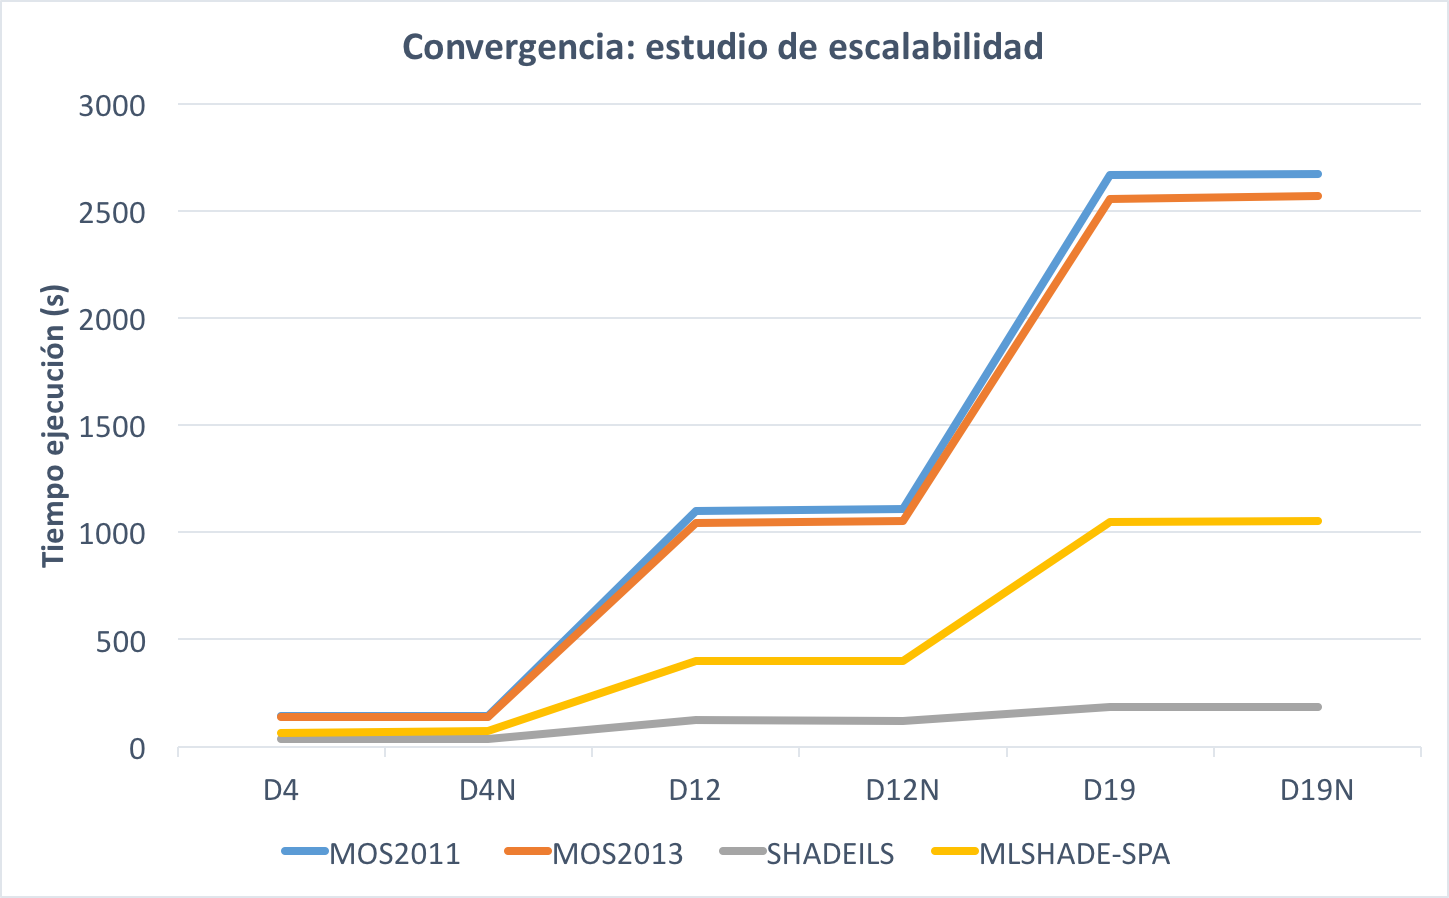
\includegraphics[scale=0.52]{imagenes/ConvergenciaEscalabilidad}
	\caption{Convergencia temporal de los 4 algoritmos para cada problema}
\end{figure}\label{fig:ConvergenciaEscalabilidad}


Atendiendo a los resultados obtenidos para los tres experimentos conducidos con DG2, se puede comprobar que el escenario obtenido no es el más indicado como para abordar el problema mediante una descomposición de variables: la salida del algoritmo, además de mostrar el excesivo tiempo de computación que emplea, muestra que no es posible realizar una descomposición del problema debido a que la función es no separable. Este escenario puede tener como explicación una razón, donde la propia naturaleza del problema puede marcar el camino del algoritmo sin necesidad de una ejecución posterior.

Como se explica en la introducción al problema, en un EEG real las señales se combinan debido a \textit{interferencias y ruido} propios de la medición, lo que hace que un electrodo \textbf{i} pueda medir información tanto local a su zona como la que se produce en otras zonas que \textbf{también} están siendo medidas por otros electrodos \textbf{k}. De esta forma, la interacción de las variables es máxima, como se puede ver en este caso, lo que limita considerablemente las capacidades del algoritmo, al no ser capaz de obtener una descomposición óptima que \textbf{minimice} la interacción entre componentes, por el simple y llano hecho de que no existe descomposición posible.

Teniendo en cuenta estos resultados y la primitiva que se expresa en \cite{DG}, la técnicas de Cooperación Co-evolutiva dedicadas a optimizar funciones no-separables de alta dimensionalidad no han mostrado resultados suficientemente competentes como para ser considerados aplicables en un ámbito real donde no se tiene información alguna acerca de la interacción de las variables de la función. A esto hay que añadirle el hecho de que los más recientes estudios de CC con descomposición de variables han sido probados con funciones separables o parcialmente separables, por lo que en gran medida se desconoce la escalabilidad de estas propuestas en funciones no-separables\cite{DG}.

Estas circunstancias motivan la decisión de \textbf{no continuar con DG2} para la fase de experimentación completa, dado que el \textbf{resultado} se torna \textbf{incierto} desde un principio y que además, las restricciones temporales inherentes al problema no pueden contemplar que una técnica híbrida que se pretende aplicar en un campo u entorno real, tenga un tiempo de respuesta superior a las \textbf{doce horas}, como es el caso de la función del EEG en el problema D12.

Teniendo en cuenta esta situación, se hace impensable la aplicación de este tipo de técnicas para optimizar un encefalograma actual que puede disponer de más de \textbf{20 señales de entrada e innumerable artifacts}, con una frecuencia de muestreo superior a la de este benchmark sintético. A partir de este punto, queda totalmente descartada la aplicación de este algoritmo en los posteriores experimentos de este estudio, por lo que tampoco se tendrá en consideración en las conclusiones finales, en cuanto a propuesta de solución real se refiere. Se procede con la fase de experimentación completa.


\section{Estudio experimental completo}\label{sect:FE2}

El estudio experimental completo muestra los resultados de 10 ejecuciones de cada algoritmo para cada uno de los 6 problemas de dimensionalidad que proponer el benchmark del EEG. En esta fase, se miden características como los valores \textbf{mínimos y máximos} de fitness alcanzados por cada algoritmo a lo largo de las 10 ejecuciones, así como una \textbf{media del fitness global} y donde, en esta ocasión, se muestra el \textbf{tiempo medio} transcurrido teniendo en cuenta la totalidad de las ejecuciones realizadas. 

En este estudio se ha utilizado un número de \textbf{evaluaciones de la función objetivo}, que es el criterio de parada, igual a 1 millón (1M); se ha elegido este valor en función de los resultados de la gráfica de convergencia destacada con anterioridad y por la escalabilidad en cuanto al tiempo de ejecución de los algoritmos. Para cada una de las técnicas, se muestra una tabla con valores \textbf{mínimos}, \textbf{máximos} y \textbf{medios de fitness} tras las 10 ejecuciones, así como el \textbf{tiempo de ejecución medio}. 

Resaltar que teniendo en cuenta que muchas de las \textbf{diferencias de valores fitness} entre los distintos algoritmos se producen más allá de las 10 cifras decimales, es posible encontrarse valores iguales tanto para mínimo, máximo y media para distintos algoritmos, fenómeno que no ocurre para las medias temporales. Posteriormente se mostrará una tabla resumen de fitness medio y tiempo medio, junto con el algoritmo de referencia, momento a partir del cual se comenzará el análisis de los resultados.

\begin{enumerate}
	\item \textbf{MOS2011}:
			
			\begin{table}[H]
				\centering
				\resizebox{\textwidth}{!}{
					$\begin{tabular}{ *{5}{c}}
					\toprule
					\textbf{Problema} & \textbf{Min.}  & \textbf{Max.} & \textbf{Media} & \textbf{Tiempo} \\
					\midrule
						D4 & 0.06103 & 0.06103 & 0.06103 & 1519.903\\ 
						D4N & 0.05897 & 0.05897 & 0.05897 & 1567.199\\ 
						D12 & 0.00194 & 0.00200 & 0.00198 & 12634.289\\ 
						D12N & 0.00187 & 0.00190 & 0.00188 & 12593.868\\ 
						D19 & 0.00830 & 0.00992 & 0.00894 & 28033.663\\ 
						D19N & 0.00824 & 0.00978 & 0.00918 & 28586.774\\ 
					\bottomrule
					\end{tabular}$
				}
					\caption{Resultados MOS2011: Experimentación completa}
					\label{tabla:ResMOS2011-Exp2}
			\end{table}
		
		\item \textbf{MOS2013}:
		
		\begin{table}[H]
			\centering
			\resizebox{\textwidth}{!}{
				$\begin{tabular}{ *{5}{c}}
				\toprule
				\textbf{Problema} & \textbf{Min.}  & \textbf{Max.} & \textbf{Media} & \textbf{Tiempo} \\
				\midrule
					D4 & 0.06103 & 0.06103 & 0.06103 & 1265.065\\ 
					D4N & 0.05897 & 0.05897 & 0.05897 & 1221.990\\ 
					D12 & 0.00194 & 0.00194 & 0.00194 & 9597.190\\ 
					D12N & 0.00183 & 0.00183 & 0.00183 & 9520.520\\ 
					D19 & 0.00251 & 0.00251 & 0.00251 & 23524.796\\ 
					D19N & 0.00256 & 0.00256 & 0.00256 & 23037.743\\ 
				\bottomrule
				\end{tabular}$
			}
				\caption{Resultados MOS2013: Experimentación completa}
				\label{tabla:ResMOS2013-Exp2}
		\end{table}
	\newpage
	\item \textbf{SHADEILS}:
	
		\begin{table}[H]
		\centering
		\resizebox{\textwidth}{!}{
			$\begin{tabular}{ *{5}{c}}
			\toprule
			\textbf{Problema} & \textbf{Min.}  & \textbf{Max.} & \textbf{Media} & \textbf{Tiempo} \\
			\midrule
				D4 & 0.06103 & 0.06103 & 0.06103 & 251.759\\ 
				D4N & 0.05897 & 0.05897 & 0.05897 & 250.908\\ 
				D12 & 0.00194 & 0.00194 & 0.00194 & 802.331\\ 
				D12N & 0.00183 & 0.00183 & 0.00183 & 786.965\\ 
				D19 & 0.00251 & 0.00252 & 0.00252 & 1578.034\\ 
				D19N & 0.00256 & 0.00256 & 0.00256 & 1573.507\\ 
			\bottomrule
			\end{tabular}$
		}
			\caption{Resultados SHADEILS: Experimentación completa}
			\label{tabla:ResSHADEILS-Exp2}
	\end{table}

	\item \textbf{MLSHADE-SPA}:

	\begin{table}[H]
		\centering
		\resizebox{\textwidth}{!}{
			$\begin{tabular}{ *{5}{c}}
			\toprule
			\textbf{Problema} & \textbf{Min.}  & \textbf{Max.} & \textbf{Media} & \textbf{Tiempo} \\
			\midrule
				D4 & 0.06103 & 0.06103 & 0.06103 & 490.294\\ 
				D4N & 0.05897 & 0.05897 & 0.05897 & 487.606\\ 
				D12 & 0.00194 & 0.00194 & 0.00194 & 3918.041\\
				D12N & 0.00183 & 0.00183 & 0.00183 & 3936.233\\ 
				D19 & 0.00252 & 0.00252 & 0.00252 & 9229.300\\ 
				D19N & 0.00256 & 0.00256 & 0.00256 & 8595.423\\ 
			\bottomrule
			\end{tabular}$
		}
			\caption{Resultados MLSHADE-SPA: Experimentación completa}
			\label{tabla:ResMLSHADESPA-Exp2}
	\end{table}
	
\end{enumerate}


\section{Comparativa Global}

La tabla resumen que se muestra a continuación permite obtener una visión global de los resultados, además de permitir comparar con el algoritmo de referencia \textbf{MAGA}\cite{MAGA-BigOpt}. En esta se aprecia el valor de fitness medio tras las 10 ejecuciones del algoritmo para cada problema. Tras discutir los resultados obtenidos en cuanto a valores fitness, se procederá con al análisis teniendo en cuenta el tiempo de ejecución.

\begin{table}[H]
	\centering
	\resizebox{\textwidth}{!}{
		$\begin{tabular}{ *{7}{c}}
		\toprule
		\textbf{Algoritmo} & \textbf{D4}  & \textbf{D4N} & \textbf{D12} & \textbf{D12N} & \textbf{D19} & \textbf{D19N}\\
		\midrule
		MOS2011 & 0.06103 & 0.05897 & 0.00198 & 0.00188 & 0.00894 & 0.00918\\ 
		MOS2013 & 0.06103 & 0.05897 & 0.00194 & 0.00183 & 0.00251 & 0.00256\\ 
		MLSHADE-SPA & 0.06103 & 0.05897 & 0.00194 & 0.00183 & 0.00252 & 0.00256\\ 
		SHADEILS & 0.06103 & 0.05897 & 0.00194 & 0.00183 & 0.00252 & 0.00256\\
		MAGA* & 0.0610 & 0.0590 & 0.0019 & 0.0018 & 0.0025 & 0.0026\\ 
		\bottomrule
		\end{tabular}$
	}
	\caption{Valores fitness medio. MAGA*: algoritmo de referencia.}
	\label{tabla:ResumenFitness}
\end{table}

A partir de los resultados obtenidos podemos deducir las siguientes conclusiones generales:

\begin{itemize}
	\item El problema \textbf{D4} (1024 variables) puede parecer más complejo de resolver a priori, en cuanto a valor fitness se refiere. Sin embargo lo que realmente ocurre es que se dispone de \textbf{menos información} - menor cantidad de señales mezcladas - de las que el algoritmo necesita para identificar la correlación entre las señales y separar los artifacts de la misma. Si además se tiene en cuenta que en un problema médico real en el que intervenga un electroencefalograma es común encontrar al menos \textbf{20 electrodos}, que actuarían como fuentes de señales, este problema no es representativo de cara a un entorno real.
	
	\item El problema \textbf{D12} (3072 variables) presenta los mejores resultados y eso se debe al equilibrio entre cantidad de información disponible y capacidad de las técnicas actuales. A pesar de crecer en términos de dimensionalidad, la calidad de las soluciones es mejor porque precisamente se dispone de mayor cantidad de información para que el algoritmo calcule la matriz \textbf{S1} con una precisión mayor que para el problema anterior. 
	
	Además cabe destacar en este punto la flexibilidad y robustez de las técnicas elegidas, debido a que a pesar de haber sido diseñadas para un benchmark cuya dimensionalidad es de 1000 variables, no pierden capacidad de convergencia frente a una dimensionalidad  3 veces mayor, llegando incluso a mostrar ajustes mejores que con menor cantidad de información. En cualquier caso, sigue siendo precipitado considerar este problema como \textit{suficientemente representativo} de un problema de optimización de un EEG real, a pesar de si ser mas representativo que el anterior.
	
	\item El problema \textbf{D19} (4864 variables) muestra como afecta la dimensionalidad del problema en la calidad de las soluciones. A pesar de alcanzar resultados bastante más satisfactorios en comparación con D4, la elevada dimensionalidad hace que a pesar de contener más información representativa para identificar la correlación entre las señales, el algoritmo no sea capaz (en términos de potencia) de obtener mejores soluciones que con menos variables. Sin embargo, se dispone de argumentos suficientes como para afirmar que las propuestas de algoritmos elegidas son \textbf{escalables}: al cambiar de benchmark han respondido de forma satisfactoria; un indicador más de la robustez de las técnicas empleadas.
	
	\item El algoritmo de referencia \textbf{MAGA} que se utiliza en esta comparativa es una técnica que, como anteriormente se ha expuesto, ha evolucionado de su antecesora y ha sido diseñada exclusivamente para la resolución del benchmark del EEG. Tomando en consideración este precepto, podemos comprobar como todos los algoritmos menos \textbf{MOS2011} (en problemas de dimensionalidad mayor, principalmente) muestran resultados prácticamente idénticos que el algoritmo de referencia, lo que es un buen indicador, nuevamente, de la potencia de estos algoritmos y las capacidades de hacer frente a problemas muy distintos.
	
	\item Finalmente, destacar que la introducción de ruido en los problemas (de varianza 0.1) no es lo suficientemente relevante como para causar un detrimento en la calidad de las soluciones, donde tampoco se ve afectado de forma significativa el tiempo de ejecución medio de los algoritmos, por lo que es importante destacar que la formulación del benchmark elegida no es la más adecuada en términos de ruido añadido, ya que no añade suficiente dificultad durante el proceso de optimización.
\end{itemize}

Tomando como referencia la tabla resumen de fitness medio (tabla \ref{tabla:ResumenFitness}), se puede comprobar como \textbf{MOS2013} introduce una mejora sustancial al cambiar el diseño del algoritmo, mejora que se hace más notable conforme crece la dimensión del problema, llegando a reducir el error obtenido en los problemas D19(N) en alrededor de un 25\% . A pesar de que la implementación de MOS2011 utiliza un algoritmo de evolución diferencial (DE) que es más escalable que el algoritmo genético clasico de MOS2013, los métodos de búsqueda local empleados por MOS2013 son mucho más potentes y rápidos, lo que le otorga a este una velocidad de convergencia superior a la de su predecesor. 

Destacar en este punto la implementación de la \textbf{MTS-LS1-Reduced} utilizada en MOS2013, donde en vez de explorar todas las variables a la vez, se centra en aquellas que más aportan a la mejora de la calidad de las soluciones, optimizando al máximo la cantidad de evaluaciones de la función objetivo a la vez que reduce la dimensión de las operaciones que realiza, otorgándole a MOS2013 mayor velocidad de convergencia, lo que se nota de forma indiscutible en las dimensiones más altas.

Si se consideran las implementaciones de \textbf{MOS2013}, \textbf{SHADEILS} y \textbf{MLSHADE-SPA} es fácilmente reconocible la potencia de las tres técnicas en comparación con MOS2011, sobretodo conforme crece la dimensionalidad del problema. Partiendo de la base de que se disponen de técnicas muy robustas y escalables, que además han mostrado rendimientos prácticamente idénticos, tanto entre ellas como con el algoritmo de referencia MAGA, se torna indispensable utilizar otro enfoque de comparativa: el \textbf{enfoque temporal}. Teniendo en cuenta que los resultados están supeditados a los tiempos de respuesta efectiva de los algoritmos, se procede a comparar las propuestas de este estudio utilizando la característica temporal, detallando en primera instancia 

\begin{table}[h]
	\centering
	\resizebox{\textwidth}{!}{
		$\begin{tabular}{ *{7}{c}}
		\toprule
		\textbf{Algoritmo} & \textbf{D4}  & \textbf{D4N} & \textbf{D12} & \textbf{D12N} & \textbf{D19} & \textbf{D19N}\\
		\midrule
		MOS2011 & 1519 & 1567 & 12634 & 12593 & 28033 & 28586\\ 
		MOS2013 & 1265 & 1221 & 9597 & 9520 & 23524 & 23037\\ 
		MLSHADE-SPA & 490 & 487& 3918 & 3936 & 9229 & 8595\\ 
		SHADEILS & 251 & 250 & 802 & 786 & 1578 & 1573\\
		\bottomrule
		\end{tabular}$
	}
	\caption{Tiempo medio (s) }
	\label{tabla:ResumenTiempo}
\end{table}


 Se parte de la idea de que, como es natural, los tiempos de ejecución están determinados por el número de variables: a mayor tamaño del espacio de soluciones, mayor cantidad de operaciones hay que realizar y más costosas se tornan estas operaciones. El ruido introducido en este benchmark, de forma sintética, no afecta de forma significativa alguna al tiempo de respuesta, llegando en ocasiones incluso a \textit{facilitar} (véase la tabla \ref{tabla:ResumenTiempo}) la convergencia del algoritmo en términos temporales. Por último,  destacar el \textbf{aumento no lineal} de los tiempos de ejecución en función del número de variables, lo que reafirma la incapacidad de obtener información alguna acerca de la correlación entre las variables de cara a una implementación híbrida de técnicas que requieran descomposiciones lo más óptimas posibles para alcanzar resultados competitivos.
 
 La tabla de porcentajes de tiempos que se muestra a continuación, que no es más que un resumen en representación porcentual de la tabla \ref{tabla:ResumenTiempo}, muestra el porcentaje de reducción temporal de cada una de las técnicas con respecto a la propuesta más lenta, en este caso, MOS2011.
 
 \begin{table}[h]
 	\centering
 	\resizebox{\textwidth}{!}{
 		$\begin{tabular}{ *{7}{c}}
 		\toprule
 		\textbf{Algoritmo} & \textbf{D4}  & \textbf{D4N} & \textbf{D12} & \textbf{D12N} & \textbf{D19} & \textbf{D19N}\\
 		\midrule
 		MOS2011 & 100 & 100 & 100 & 100 & 100 & 100\\ 
 		MOS2013 & 83 & 77 & 75 & 75 & 83 & 80\\ 
 		MLSHADE-SPA & 32 & 31& 31 & 31 & 32 & 30\\ 
 		SHADEILS & 16 & 15 & 6 & 6 & 6 & 5\\
 		\bottomrule
 		\end{tabular}$
 	}
 	\caption{Porcentaje (\%) de reducción temporal }
 	\label{tabla:ResumenTiempoPorcentaje}
 \end{table}

A través de esta tabla se puede comprobar como \textbf{MOS2013} tiene un mejor tiempo de respuesta que su antecesor MOS2011. Las técnicas de búsqueda locales empleadas por este son más potentes que las de su predecesor, lo que se traduce también en un tiempo de respuesta menor: MOS2013 consigue reducir los tiempos de ejecución entre un 20\% y 25\% con respecto a MOS2011 para la totalidad de los problemas.

En cuanto al segundo mejor, en términos temporales, \textbf{MLSHADE-SPA} tiene un rendimiento destacable frente a las dos propuestas MOS. Emplea alrededor de un 30\% del tiempo que necesita MOS2011 y menos de la mitad del que requiere MOS2013, llegando a resolver el problema de dimensión D12 en una hora en vez de 3, al igual que emplea de media algo menos de 3 horas en resolver el problema D19, tiempo que en MOS2013 se va hasta rozar las 8 horas de ejecución.

A grandes rasgos, queda muy claro que \textbf{SHADEILS} es el mejor de todos los algoritmos en relación calidad de la solución - tiempo de ejecución, donde se mantiene a menos de un 10\% del tiempo de ejecución que emplea MOS2011 para los problemas D12(N) y D19(N). La diferencia con MOS2013 es un poco menos significativa, en torno a un 12.5\% de media para todos los problemas, y cerca de un 20\% del tiempo con respecto a MLSHADE-SPA para dimensiones D12 y D19, situándose como claro vencedor en esta comparativa dado que es \textbf{único algoritmo} que ha conseguido resolver todos los problemas en menos de media hora.


Sin embargo, estos resultados pueden parecer contradictorios a priori debido a la \textbf{naturaleza de las implementaciones} y de las \textbf{tecnologías empleadas}. Es bien sabido que \textbf{C++ y C} son los lenguajes de programación \textbf{más rápidos} de la actualidad, dada su condición de \textit{compilados}. Seguidamente, otros lenguajes como pueden ser en este caso \textbf{Python} o \textbf{MATLAB} quedan forzosamente por detrás de C++ al ser lenguajes interpretados. Surge entonces la pregunta de cómo una implementación en un lenguaje compilado, como las de MOS2011 y MOS2013, es ordenes de magnitud \textbf{más lenta} que una implementación en un lenguaje interpretado, como las de SHADEILS y MLSHADE-SPA.

La respuesta está en el diseño de cada una de las técnicas. Mientras que tanto MOS2011 como MOS2013 utilizan la librería \textbf{GAlib}, que a grandes rasgos no es más que un conjunto de plantillas para diseñar algoritmos evolutivos, pero que añade mucha complejidad estructural al algoritmo además de la propia que ya introduce el diseño del algoritmo en cuanto a parámetros propios y las operaciones que efectúa, SHADEILS hace un uso intensivo de librerías como \textbf{Numpy}, que permiten acceder desde Python a implementaciones robustas y optimizadas de operaciones en C++, consiguiendo un resultado en cuanto a tiempo de respuesta muy similar al que se obtendría si se utilizase C++ de forma nativa.

Siguiendo con el diseño, MOS utiliza algoritmos evolutivos clásicos como el \textbf{GA}, cuya escalabilidad es muy baja, lo que aumenta considerablemente el tiempo de ejecución. Por otra parte, tanto SHADEILS como MLSHADE-SPA hacen uso intensivo de técnicas muy avanzadas de evolución diferencial, como lo es \textbf{SHADE} o \textbf{L-SHADE}, esta última presente en MLSHADE-SPA donde aplica una reducción gradual de la población. Aunque no es posible saber con certeza si un tamaño de población que se reduce constantemente pueda ser indicativo de una mejora en el tiempo de respuesta, como es el caso si se comparan MOS y MLSHADE-SPA, hay que tener en cuenta que SHADEILS utiliza apenas un cuarto de la población de MOS2013, lo que si puede ser indicativo de una mejora sustancial de un algoritmo a otro.

Dada la implementación particular de cada técnica y los resultados obtenidos al utilizar distintos lenguajes de programación, se puede afirmar que si se implementasen todas las técnicas en un mismo lenguaje, prevalecerían los resultados que se han obtenido en este estudio, consiguiendo reducir aún más los tiempos de ejecución de algoritmos como SHADEILS o MLSHADE-SPA. 

No obstante, si ahora se compara a SHADEILS con el algoritmo de referencia \textbf{MAGA}, los resultados no parecen ser tan competitivos. MAGA es un algoritmo que ha sido diseñado expresamente para este benchmark, por lo que no se tienen registros algunos de resultados con otros benchmarks del panorama LSGO. Además, el autor de la publicación no refleja el criterio de parada del algoritmo ni la cantidad de evaluaciones de la función objetivo que ejecuta, por lo que se ha tomado la decisión de medir el tiempo que tarda \textbf{SHADEILS} en alcanzar una \textbf{precisión igual} a la que se muestra en el algoritmo de referencia en cuanto a valor fitness, para así poder comparar ambos algoritmos bajo condiciones similares.

Para ello, se ha ejecutado SHADEILS para cada problema con una semilla aleatoria y 1 millón de evaluaciones de la función objetivo. La tabla correspondiente se muestra a continuación, donde los valores fitness de referencia que se han utilizado para esta experimentación en concreto son los que aparecen en la tabla \ref{tabla:ResumenFitness}.

\begin{table}[h]
	\centering
	\resizebox{\textwidth}{!}{
		$\begin{tabular}{ *{7}{c}}
		\toprule
		\textbf{Algoritmo} & \textbf{D4}  & \textbf{D4N} & \textbf{D12} & \textbf{D12N} & \textbf{D19} & \textbf{D19N}\\
		\midrule 
		SHADEILS & 1.152 & 0.934 & 47.175 & 47.759 & 472.229 & 472.010\\ 
		MAGA & 0.190 & 0.191 & 1.322 & 1.396 & 7.176 & 9.216\\ 
		\bottomrule
		\end{tabular}$
	}
	\caption{Tiempo (s) de SHADEILS en conseguir un error igual a MAGA }
	\label{tabla:ResumenMAGA-SHADEILS}
\end{table}

Los datos muestran que SHADEILS tiene una velocidad de convergencia alta, hecho que queda demostrado tras haber medido el tiempo transcurrido hasta que se alcanza por primera vez la solución optima de MAGA. Si se tiene en consideración que el autor de la publicación ha utilizado Visual Studio 2010 y Windows 7 para la implementación de la propuesta\cite{MAGA-BigOpt}, es posible que también haya utilizado C++ para la implementación del algoritmo. Tomando en cuenta las consideraciones expresadas anteriormente en cuanto a la mejora de tiempo que se conseguiría al trasladar la implementación de los algoritmos de MATLAB y Python (MLSHADE-SPA y SHADEILS respectivamente) existe una alta probabilidad de que los tiempos de respuesta de estos algoritmos también mejoren, lo que reduciría las distancias actuales entre SHADEILS y MAGA, situando al primero de estos en una muy buena posición con respecto a sus demás competidores.

Llegados a este punto es apropiado afirmar que las propuestas elegidas en este estudio han mostrado resultados competitivos. Aún así se puede concluir que son necesarias técnicas no más potentes pero si \textbf{más rápidas} para permitir su aplicación sobre problemas de optimización en ámbitos reales. El campo LSGO es un área de conocimiento que ha nacido relativamente hace poco y hasta hace apenas tres años, la gran mayoría de propuestas se remitían únicamente a los congresos, conferencias y competiciones, siendo estudiadas y evaluadas sobre benchmarks poco representativos del panorama del LSGO del mundo real. 

Sin embargo, durante los últimos tres años se han propuesto una mayor cantidad de técnicas y algoritmos en este campo de estudio, lo que indudablemente promoverá su crecimiento y evolución de forma notable. Además, permitirá que sea solo cuestión de tiempo que se propongan técnicas mucho más sofisticadas y potentes que lleguen a ser aplicables a un problema real, repercutiendo en una mejora de la calidad de los procesos que requieren optimización y por ende afectando de forma positiva al entorno social donde son implantadas.












